\documentclass{dalcsthesis}
\usepackage{fullpage}
\usepackage{textcomp}
\usepackage{graphicx}
\usepackage{algorithm}
\usepackage{algorithmic}
\usepackage{amsthm}
\newtheorem{lemma}{Lemma}
\usepackage{amsfonts}
\usepackage{amsmath}

\title{Rational Secret Sharing with and without Synchronous Broadcast, Conspicuous Secrets, Malicious Players and Unbounded Opponents}
\author{Craig Gidney}
\date{\today}
\defenceday{_______________________________XXXXXXXXXXXX______________________}
\defencemonth{January}
\defenceyear{2012}

\begin{document}
\mcs
\maketitle

\chapter{Introduction}

Secret sharing allows some data $s$ to be split into $n$ shares such that any set of $t$-1 shares reveal no information about $s$ but any set of $t$ shares can be used to easily compute $s$. Shamir \cite{shamir79} elegantly solved this problem in 1979 using polynomials over finite fields. However, recent interest \cite{fuch10, ong09, kol08, maleka08, abraham06, gordon06} has focused on the practical issues of recombining shares of a secret in the presence of adversarial players.

This paper presents protocols, and bounds on the effectiveness of any protocol, for recombining secrets in the presence of players who do not want others to learn the secret (rationality), may not want to learn the secret themselves (maliciousness), may be colluding, may have unbounded computational capacity, may not be able to synchronize sends (synchronous broadcast), and/or may be able to recognize the secret independently (conspicuousness).

\section{The Landscape of Rational Secret Sharing}

Different secret sharing protocols target different types of players and apply different assumptions. We review these definitions, some from the literature and some defined by this paper, since this paper uses them extensively.

\subsection{Rational Player}

In secret sharing, rational players are not just rational in the economic sense of maximizing utility. They have specified preferences \cite{halpern04}: they want to learn the secret but, secondarily, want to prevent others from learning the secret. Secret sharing protocols incentivize rational players into cooperating by ensuring defecting decreases the probability of learning the secret by a large enough amount.

A protocol that works in the presence of rational players is more applicable to the real world than a protocol that doesn't. For example, consider a group of financial firms with shares to valuable market information. Each firm would profit from access to the information but would profit even more from exclusive access. Since firms benefit the most from exclusive access to the secret, they are rational in the secret sharing sense. If the firms attempt to combine their shares of the secret using a protocol that assumes players will cooperate, one of them may defect and gain exclusive access. That possibility may prevent the firms from even attempting to combine their shares.

A rational player's payoff is guaranteed to be larger if they learn the secret but that doesn't mean they ignore their secondary preference. They may be willing to trade a small decrease in the probability of learning the secret in exchange for a large increase in the probability of others not learning the secret. Rational secret sharing protocols need to account for these tradeoffs.

A rational player who has learned the secret is effectively malicious. They want to prevent others from learning the secret and don't care about learning the secret, because they already know it.

\subsection{Malicious Player}

Malicious players only care about preventing other players from learning the secret. They want the process of learning the secret to be delayed, aborted, and corrupted. They can't be incentivized into cooperating. Instead, their actions must be authenticated and constrained.

Even if there are enough honest players to meet the share threshold, a few unchecked malicious players can prevent a protocol from succeeding. If 10 out of 100 shares are faked, the probability of choosing a subset of 80 authentic shares at random is about $3.4 \times 10^{-16}$. It could take centuries at millions of attempts per second to find a valid subset by brute force.

\subsection{Coalition}

Coalitions are groups of players working together to further their collective goals. The larger a coalition is, especially as its size approaches the number of players $n$ or the threshold $t$, the more powerful it becomes.

Coalitions of rational players are limited to $t-1$ members. Larger rational coalitions have enough shares to learn the secret without help, so they do and become malicious. Coalitions of malicious players can have up to $n-1$ members. Malicious coalitions with more than $n-t$ players can trivially prevent the secret from being learned by not participating, but may attempt to go further and cause the wrong secret to be learned.

\subsection{Interactive Dealer}

An interactive dealer is available to the players when shares are being combined. For example, several papers \cite{halpern04, gordon06, maleka08} include protocols where the dealer re-issues new shares of the secret on demand.

Having an interactive dealer simplifies secret sharing considerably. In fact, if the dealer is not limited to just re-issuing shares, the problem becomes trivial: the dealer accepts votes to reveal the secret and does so when the number of votes exceeds the threshold.

Note that a dealer with the ability to generate shares but the inability to count votes is not necessarily absurd. The dealer may be a simulation within a multi party computation, with restrictions on possible computation due to security or performance concerns.

All the results in this paper assume a non-interactive dealer who issues shares once and then disappears.

\subsection{Honest Dealer}

A dealer is honest if they generate valid and unbiased shares. In contrast, a dishonest dealer may create shares that always favor a particular player or do not ensure a termination condition occurs. Note that we do not consider whether or not the dealer creates shares for the ``correct" secret, because the secret's correctness if outside of the secret sharing protocol's control.

The presentation of the protocols in this paper assume the dealer is honest. But the following two methods, where applicable, can ensure unbiased shares and detect invalid shares and allows us to relax the assumption:

\begin{itemize}
  \item The dealer commits to the shares but before shares are distributed the players shuffle the share-to-player mapping. This shuffling prevents the dealer from biasing the protocol against a chosen subset of players.  
  \item The dealer commits to shares of a random secret but, before the shares are distributed, the players choose to either check or accept. If they choose to check then the dealer reveals the entropy used to generate the shares and the random secret. The players can't verify the entropy is ``random" but they can verify that using it generates shares matching the commitments. This proves the shares were not malformed because the protocol may generate them when followed correctly. After the check is completed, the dealer generates more shares and the process repeats until the players choose to accept. In that case the dealer distributes the shares and reveals the offset from the shared secret to the true secret. This check-or-accept process prevents the dealer from undetectably creating invalid or malformed shares.
\end{itemize} 

\subsection{Synchronous and Asynchronous Broadcast}

Synchronous broadcast is the ability for players to send their messages (or commit to not sending messages) for a round before being able to receive any other player's message(s) for that round. Additionally, synchronous broadcast implies all players receive the same message in a timely and reliable fashion. Players can't send different messages to different players and players do not have to differentiate between a delayed message and a missing message. 

Asynchronous broadcast provides the same reliability, timeliness, and broadcast guarantees as synchronous broadcast but does not allow players to synchronize when they send the messages. If multiple players are supposed to send at the same time, some of them can receive messages before they send their own message. As a consequence, message orderings need to be explicit. Otherwise the protocol is prone to deadlock because rational players have an incentive to wait to receive before sending. For example, if rational players A and B are combining a secret and they believe the next round of messages could be the last round then they both want to wait to receive the other player's message before sending their own because, if it is the last round, they could then defect and learn the secret while preventing the other player from learning it. 

This paper presents protocols for both synchronous and asynchronous broadcast and also shows that asynchronous protocols are inherently weaker than synchronous protocols, such as requiring a sacrificial player when the secret is conspicuous. Weakening other assumptions, like the broadcast assumption that players can't send conflicting messages to different players, are left for future work.

\subsection{Bounded and Unbounded Players}

Unbounded players can perform any desired finite number of computations within a fixed time. They can trivially break schemes relying on computational difficulty, like reversing one way functions, but can't defeat schemes secure in the information theoretic sense, like encryption with a one-time-pad or Shamir's Secret Sharing Scheme \cite{shamir79}.

This paper proposes protocols for both bounded and unbounded players. Protocols that work in the presence of unbounded players are secure in the stronger information theoretic sense but can't rely on tools like secure pseudo random number generators.

\subsection{Conspicuousness of the Secret} 

This paper defines a secret to be conspicuous if, given a guess at the secret, it is possible to determine if the guess is correct. For example, the combination to a lock is conspicuous because, given a combination, you can check if it works. The combination can be brute forced, given enough time. Conversely, the combination to a ``burn safe", which destroys itself and its contents if the wrong combination is entered, is almost entirely inconspicuous. The combination can't be brute forced.

Any secret can trivially be made conspicuous using a bit commitment, but returning to inconspicuousness is impossible. A secret sharing protocol for inconspicuous secrets may start by making the secret conspicuous, but this is a tradeoff. Conspicuousness prevents the wrong secret from being accepted, by allowing it to be checked, but allows unbounded opponents to brute force the secret and, as shown later, requires a player to be sacrificed if communication is asynchronous.

Conspicuousness can be relative to the player or group of players. A secret may be conspicuous to one player but inconspicuous to another. It may be conspicuous to a pair of players but inconspicuous to each individually. Once a secret sharing protocol starts the secret must be at least conspicuous to groups of players over the threshold size, because by definition they can compute the secret. This paper, when refering to conspicuousness, implicitely refers to the original conspicuousness of the secret, before the protocol started, unless otherwise noted.

\subsection{Temptation}

Temptation, introduced by this paper, is a measure of how much a rational player or coalition can benefit from defecting. We define it as the expected probability a rational player or coalition, who does not know the secret, has of learning the secret if they unilaterally defect now (stop following the protocol as expected). Bounding temptation allows a protocol to ensure rational players without a strict preference for learning the secret will not defect.

A protocol has constant temptation if the temptations encountered by players and coalitions, until they learn the secret, are all equal.

A protocol's maximum temptation is the largest temptation that can be encountered by a player or coalition. The naive protocol, where players just broadcast their share, has a maximum temptation of 1. If a single player defects then they will learn the secret with probability 1. A round-based protocol where a single round has probability $x$ of being the final round has a maximum temptation of at least $x$.

Some protocols have maximum temptations that are dependent on the shares generated by the dealer. In particular, there may exist a ``bad deal" that is possible but unlikely. In those cases, this paper distinguishes between worst deal maximum temptation, the maximum of the maximum temptations over all possible deals, and expected deal maximum temptation, the average of the maximum temptations weighted by the likelihood of possible deals.

\subsection {Immunity}

A protocol is immune to rational players or rational coalitions if it causes them to cooperate until they learn the secret. This occurs when, even if malicious players may be present, cooperating is a Nash equilibrium. Informally: protocols immune to rational players turn rational players into cooperating players (until they learn the secret).

A protocol is immune to malicious players or malicious coalitions if it can, with arbitrarily high probability, achieve the same outcome as if they had not been present. Informally: protocols immune to malicious players turn malicious players into absent players.

This paper refers to protocols that are immune to both rational and malicious coalitions as ``coalition immune".

\section{Document Map}

[map of the rest of document]




\chapter{Related Work}
\label{sec:RelatedWork}

In 1979 Adi Shamir published the paper 'How to Share a Secret' \cite{shamir79}, detailing how to divide a secret into $n$ shares with a threshold $t$ such that any set of $t$ shares can easily reconstruct the secret but fewer than $t$ shares provided no information about the secret. In Shamir's scheme, shares are points on an up-to-$(t-1)$'th degree polynomial over a finite field of size $p$. The secret is the polynomial's value at $x=0$. An up-to-$(t-1)$'th degree polynomial can be interpolated from any set of $t$ points. But if only $t-1$ points are known then there is exactly one matching polynomial for each possible value at $x=0$ and the next share can cause the secret to be any value. Thus an attacker with $t-1$ shares has no more information about the secret than an attacker with $0$ shares. The scheme is secure in the information theoretic sense.

The rational secret sharing problem was introduced by Halpern and Teague in their 2004 paper 'Rational Secret Sharing and Multiparty Computation' \cite{halpern04}. They showed that, if all players are rational, prefering to learn the secret but secondarily prefering others to not learn the secret, then there is no protocol with bounded worst-case completion time. If a protocol definitely ends after round $k$ then rational players have no incentive to send a message on round $k$, meaning there is no incentive to send a message on round $k-1$ because there will be no reciprocation in round $k$, and so forth.

Halpern and Teague present a 3-of-3 protocol with bounded \emph{expected} time. The protocol bypasses the impossibility result by terminating probabilistically. The protocol is divided into rounds started by the dealer giving the players a new set of shares for the secret. The players then effectively flip coins while satisfying the constraint that the number of coins coming up heads is not equal to 2 and also allowing checking the flips after the fact. Players transmit their share if their coin comes up heads. The number of heads is constrained from being 2 to prevent only one player from learning the secret if only the other two players broadcast their shares. Rational players are incentivized to cooperate because, given that a rational player flips heads, the other two players may have flipped tails and not sending in that case means the other players will stop participating. They also explain how to extend the coin flip protocol to other thresholds and numbers of players, except for the $2$-of-$2$ case.

The paper 'Games For Exchanging Information' \cite{kol08} by Kol and Naor in 2008 presents two protocols for rational non-colluding players with synchronous broadcast and an inconspicuous secret. They avoid cryptographic primitives, like one way functions, arguing that they implicitely bound the number of rounds and thus cause rational players to defect. As a result, their protocol does not rely on computational difficulty and works equally well for unbounded players.

Their first protocol is for the 2-of-2 case. The dealer generates a short list of random entries with random length following a geometric distribution and a long list starting with the short list, followed by the secret, and then random entries with random length following the same geometric distribution. Each round players send the next entry in their list. If the sent values do not match, the protocol is aborted. If one player does not send a value, it is assumed they were the short player and the single sent value is the secret. The second protocol is for the general $t$-of-$n$ case. In this augmented protocol every player but one gets the long list, list entries include authentication information as well as $t$-of-$n$ shares of an 'indicator' flag which allows subsets without the short list to notice the final round, and future list entries must be unmasked using shared information from previous rounds.

As remarked in the paper, Kol and Naor's generalized protocol is susceptible to coalitions. If a coalition includes the short player then they know the last round and can betray the other players. If the coalition does not include the short player then they know a slightly stricter upper bound on the final round than a single player would, meaning that in the case where the long lists are at the minimum possible length they will know when the final round occurs and can betray the other players.

Kol and Naor remark that their 2-of-2 protocol is not dependent on synchronous broadcast, as long as the dealer predefines the order messages must be sent and includes authentication. The long player sends first on the definitive round. The short player, knowing it is the definitive round because their list has run out, knows the secret is the sent message. Then, because the short player has no authenticated messages to send, the long player does not receive a valid message and concludes it is the definitive round and knows the secret is the current item in their list.

Another paper on rational secret sharing is the 2009 'Fairness with an Honest Minority and a Rational Majority' \cite{ong09} by Shien Jin Ong, David C. Parkes, Alon Rosen, and Salil Vadhan. This paper sidesteps Helpern and Teague's impossibility result by assuming the presense of a small minority of honest players. They present an asynchronous single-round $t$-of-$n$ protocol with probabilistic success where the first $t-1$ players (the 'starters') broadcast their share and the remaining players (the 'finishers') broadcast their share only if all of the starters cooperated. Rational finishers will defect but honest finishers will cooperate as long as all of the starters cooperated. Rational starters are incentivized into cooperatubg by the chance of there being an honest finisher. Thus the $t-1$ starters will broadcast their share, ensuring the finishers learn the secret, and if there is an honest finisher they will broadcast their share and the starters will learn the secret.

In 2010 Georg Fuchsbauer, Jonathan Katz and David Naccache published 'Efficient Rational Secret Sharing in Standard Communication Networks' \cite{fuch10}. They present a synchronous protocol for inconspicuous secrets that uses verifiable random functions to blind secret shares until a target round and indicator shares until the next round. When players find the unblinded indicator shares combine to form 0 they know the previous round's unblinded secret shares form the secret.

We use techniques from the 2010 paper, extending them to work with malicious players, conspicuous secrets, unbounded opponents and asynchronous broadcast. Note that the 2010 paper claims its synchronous protocol works asynchronously by asserting players only find out about the target round during the following round. But players can use the fact that the unblinded secret shares are random during rounds that aren't the target round in order to detect it. For example, if there are 4 rational players, 2 of which are colluding, and the threshold is 3 then the coalition can wait to receive the 2 non-colluding players' shares then interpolate a polynomial from the 4 shares they have. If the polynomial has degree 3 then the 4 shares are not consistent with a 3-of-4 shamir scheme, meaning the target round is not occuring. Otherwise it is the target round with high probability and the colluders will defect, learning the secret while preventing the other players from learning the secret.

Other papers on rational secret sharing include 'Rational Secret Sharing with Repeated Games' \cite{maleka08}, which proposes an asynchronous protocol requiring an interactive dealer, 'Cryptography and game theory: Designing protocols for exchanging information' \cite{kol08-2}, which proposes a synchronous protocol and an asynchronous protocol based on secure multi-party computation and meaningful/meaningless encryption, and 'Distributed Computing Meets Game Theory: Robust Mechanisms for Rational Secret Sharing and Multiparty Computation' \cite{abraham06}, which proposes a protocol based on simulating an interactive dealer using multi-party computation.

Finally, several cryptographic primitives are useful for efficient rational secret sharing. Bit commitment \cite{naor91} allows the dealer to give players the ability to check if they have the right secret. Verifiable random functions (VRFs) \cite{micali99, dis05} allow a sequence of deterministic and verifiable messages to be created from a small seed. In examples this paper will use plain sha1 and RSA for bit commitment and verifiable random functions, but these basic primitives are used for their simplicity, not their security.




\chapter{Synchronous Broadcast}

Synchronous broadcast allows players to assume the messages they send during a round $r$ can't be received by other players before they send their own messages for round $r$. This allows simpler and more efficient protocols than with asynchronous broadcast.

In this chapter two synchronous protocols are presented: one for bounded opponents and one for unbounded opponents. [Summarize Results\ldots]



\section{Synchronous Protocol for Bounded Opponents achieving Coalition Immunity}

We propose a protocol that assumes synchronous broadcast and bounded opponents, hereafter referred to as ``SBP'' (synchronous bounded protocol). Assuming synchronous broadcast and bounded opponents allows several simplifications. For example, the secret can be made conspicuous without any cost to security, implicitely protecting players from being fooled into accepting the wrong secret.

Like many rational secret sharing protocols \cite{halpern04, kol08, fuch10}, SBP is based on a sequence of check rounds followed by a definitive round where every player simultaneously learns the secret. Each round every player sends a message created by a verifiable random function (VRF). The messages are then added to player specific offsets to create round shares. Both the offsets and VRFs are chosen beforehand by the dealer. Before the definitive round the round shares are random but on the definitive round the round shares are the Y coordinates of Shamir shares for the secret with a threshold of $t$, because of how the offsets and VRFs are chosen by the dealer. Players recognize the definitive round by combining the round shares and matching the result against a bit commitment to the secret provided by the dealer. See Algorithms \ref{alg:SBP:Dealer} and \ref{alg:SBP:Player} and Figure \ref{ex:SBP} for details.

A similar protocol has been proposed by Fuchsbauer et al. \cite{fuch10} but there are important differences. First, Fuchsbauer et al. have players detect the definitive round by using additional round indicator shares. When the round indicator is 0 the previous round's secret shares combine to reveal the inconspicuous secret. SBP uses a bit commitment instead of round indicator shares because, as explained in Section \ref{sec:RelatedWork}, the indicator shares are mostly redundant. Second, Fuchsbauer et al.'s protocol is only intended to work with rational players and aborts if any player defects. SBP works with rational and malicious players and, to prevent a single malicious player from trivially ending the protocol, continues until the number of remaining cooperating players drop below the threshold necessary to reconstruct the secret. Finally, Fuchsbauer et al. claim their protocol also works in the asynchronous case whereas this paper presents a different protocol for that case.

\begin{algorithm}
  \caption{Dealer Protocol for SBP}
  \label{alg:SBP:Dealer}
  \begin{algorithmic}[1]
    \INPUT Total number of shares $n$ and threshold $t$
    \INPUT Marginal probability $\alpha$ of the definitive round occuring
    \INPUT Verifying function scheme $VRFS$
    \INPUT Commitment scheme $CS$
    \INPUT Finite field $\mathbb{F}$
    \INPUT Secret value $s$ from the finite field $\mathbb{F}$
    \OUTPUT An ordered list of $n$ SBP Shares containing offsets, public keys, a private key, a commitment, and an index
    \STATE Create a commitment $c$ to the secret
    	$$c = CS.CreateCommitmentTo(s)$$
    \STATE Create ordered lists $V$ and $G$ of $n$ public ($V$) and private ($G$) VRFS key pairs
    	$$V_i, G_i = VRFS.NewKeyPair()$$
    \STATE Choose the random definitive round $r$ from a geometric distribution with marginal probability $\alpha$
    \STATE Create an ordered list $S$ of $n$ Shamir shares $S_i$ where $i > 0$ with threshold $t$ for the secret
    	$$S = CreateShamirShares(s, \mathbb{F}, n, t)$$
    	$$XOfPoint(S_i) = i$$
    \STATE Compute the ordered list $Y$ of $n$ offsets $X_i$
    	$$Y_i = YOfPoint(S_i) - VRFS.ValueOf(G_i, r)$$
    \STATE Return the list $R$ of $n$ shares composed of the commitment, all public keys, all offsets, an index, and a private key
    	$$R_i = (c, V, Y, i, G_i)$$
  \end{algorithmic}
\end{algorithm}

\begin{algorithm}
  \caption{Player Protocol for SBP}
  \label{alg:SBP:Player}
  \begin{algorithmic}[1]
    \INPUT Total number of shares $n$ and threshold $t$
    \INPUT Verifying function scheme $VRFS$
    \INPUT Commitment scheme $CS$
    \INPUT Finite field $\mathbb{F}$
    \INPUT Share Index $i > 0$
    \INPUT VRFS private key $G_i$
    \INPUT Ordered list $V$ of $n$ VRFS public keys
    \INPUT Ordered list $Y$ of $n$ offsets
    \INPUT Secret commitment $c$
    \OUTPUT Secret Value or Failure
    \STATE Mark all players, identified by indexes in $[1, n]$, including ourselves, as cooperating
    \STATE Let $r = 1$
    \WHILE { true }
      \STATE Send the round message $M_i = VRFS.ProofAndValueOf(G_i, r)$ to all cooperating players, including ourselves
      \STATE Receive round messages. Let $M_j$ be the message or lack of message from player $j$.
      \STATE Mark any messages $M_j$ that do not pass $VRFS.Verify(V_j, M_j)$ as invalid
      \STATE Mark players that sent no message or an invalid message as non-cooperating
      \STATE Discard messages from non-cooperating players
      \STATE If the number of cooperating players is less than $t$ then exit with failure
      \STATE Compute the round share of each cooperating player with index $j > 0$
			$$S_j = Point(j, M_j.Value + Y_j)$$
      \STATE Combine any set $S'$ of $t$ of the known round shares to get the potential round secret $s$
      		$$s = ShamirCombine(S', \mathbb{F}, n, t)$$
      \STATE If $CS.Matches(c, s)$ is true then exit with $s$ as the secret value
      \STATE Increment $r$ by 1
    \ENDWHILE
  \end{algorithmic}
\end{algorithm}

\begin{figure}
  \caption{Example run of SBP}
  \label{ex:SBP}
  \begin{itemize}
    \item Finite Field $\mathbb{F}$ is integers mod 5
    \item Share Count $n = 2$
    \item Threshold $t = 2$
    \item Marginal round termination probability $\alpha = \frac{1}{3}$
    \item Verifiable Random Functions $PedagogicalRSA(p: 7, q: 11)$
    \item Commitment Scheme $CS = PlainSHA1$
    \item Secret $s = 3$
    \item Create commitment $c = CS.Create(s) = 0x984292\ldots$
    \item Create RSA key pairs for VRFS for each of the 2 players
    \subitem $V_1, G_1 = 17, 53$
    \subitem $V_2, G_2 = 13, 37$
    \item Pick the definitive round $r = 3$
    \item Create the Shamir shares $S_i$ for each player based on a generated polynomial $P$
    \subitem $P(x) = 3 + 4x \pmod{5}$
    \subitem $S_1 = (1, 2)$, $S_2 = (2, 1)$
    \item Compute the offsets 
    \subitem $X_1 = 2 - (3^{53} \pmod{77}) \equiv 2 \pmod{5}$
    \subitem $X_2 = 1 - (3^{37} \pmod{77}) \equiv 0 \pmod{5}$
    \item Start player protocol 
  \end{itemize}
  \begin{tabular}{|r|r|r|r|r|}
    \hline
    Round & Msg mod $77$   & Check mod $77$ & Round share mod $5$    & Combine mod $5$\\
    \hline
    1 & $M_1 = 1^{53} = 1$  & $1^{13} = 1$   & $P(1) = 1+2 = 3$  & $P(x) = 0 + 3x$\\
      & $M_2 = 1^{37} = 1$  &  $1^{17} = 1$  & $P(2) = 1+0 = 1$  & $Match(0, c)$: False\\
    \hline
    2 & $M_1 = 2^{53} = 74$ & $74^{13} = 2$  & $P(1) = 74+2 = 1$ & $P(x) = 1$\\
      & $M_2 = 2^{37} = 51$ &  $51^{17} = 2$ & $P(2) = 51+0 = 1$ & $Match(1, c)$: False\\
    \hline
    3 & $M_1 = 3^{53} = 5$  & $5^{13} = 3$   & $P(1) = 5+2 = 2$  & $P(x) = 3 + 4x$\\
      & $M_2 = 3^{37} = 31$ & $31^{17} = 3$  & $P(2) = 31+0 = 1$ & $Match(3, c)$: True\\
    \hline
  \end{tabular}
\end{figure}


\subsection{Analysis}

SBP has reasonable performance: comparable to Shamir's scheme with signed shares. If the number of players is $n$, the threshold is $t$, the marginal definitive round probability is $\alpha$, and the costs of the verifiable random function scheme and Shamir's share scheme are represented as $VRFS$ and $Shamir(t, n)$ then the asymptotic time is $O(VRFS \times n + Shamir(t, n))$ for the dealer and $O(\frac{1}{\alpha} \times (VRFS \times n + Shamir(t, n)))$ for the players. The practical costs depend primarily on the efficiency of the implementations of the VRF and Shamir schemes.

SBP's shares each contain $O(n)$ information, but most of it (the commitment, the VRF public keys and the offsets) is common to all of the shares. The amount of unique information in each share (the index and the VRF private key) has constant size. Reducing the amount of common information would require a radically different authentication method.

SBP is coalition immune, as shown in Lemma \ref{Lem:SBPMalImmune} and Lemma \ref{Lem:SBPRatNash}. Coalitions of any size do not gain any advantages except those required by the nature of secret sharing. Rational coalitions up to the maximum size $t-1$ will cooperate until they learn the secret. Malicious coalitions up to size $n-t$ can't prevent players from learning the secret. Malicious coalitions up to size $n-1$ can't convince players to accept the wrong secret.

If SBP is run with $t$ or more rational players then they will learn the secret, even in the presence of malicious players, with arbitrarily high probability. This is a consequence of coalition immunity. We know the malicious players can be treated as absent players and the rational players will cooperate until they learn the secret. Since there are enough cooperating players and they all learn the secret at the same time, the rational players will learn the secret.

\begin{lemma} SBP has constant temptation $\alpha$ \label{Lem:SBPConstTempt} \end{lemma}
\begin{proof}
A defector only learns the secret if they defect during the definitive round. If they defect earlier then the other players will stop cooperating with them and they won't receive the round shares necessary to learn the secret on the definitive round. They can't defect later because the protocol ends after the definitive round. 

To check if a round is the definitive round, $t$ round shares are needed. Before a round, rational players and coalitions have fewer than $t$ round shares. Therefore rational players and coalitions can't detect the final round until after it has occured. All they know is the marginal probability of each round being the definitive round: $\alpha$. Therefore a rational player or coalition always believe defecting will give them the secret with probability $\alpha$.
\end{proof}

\begin{lemma} SBP is immune to malicious players and coalitions \label{Lem:SBPMalImmune} \end{lemma}
\begin{proof}
Malicious players will defect before or during the definitive round, because otherwise the other players will have more definitive round shares and will be more likely to learn the secret. In SBP players defect by sending no round message or by sending a fake round message.

If a player sends no round message then they are marked as non-cooperating by all cooperating players (see Algorithm \ref{alg:SBP:Player}). If a player sends a fake message then they are detected, with arbitrarily high probability bounded by the security of the VRF scheme, and marked non-cooperating by all cooperating players. Coalitions have multiple chances to send a fake message, but the probability of all the fake messages being detected is still arbitrarily high based on the VRF scheme. 

A player that has been marked non-cooperating by all cooperating players is effectively absent from the protocol. They are sent no messages and the messages they send are discarded. Because rounds don't depend on information from previous rounds, the protocol will terminate as if it had started without the non-cooperating players being present.

Therefore, with arbitrarily high probability, a malicious player or coalitions's effect on the outcome of the protocol is equivalent to that of an absent player.
\end{proof}

\begin{lemma} By choosing a small enough $\alpha$, SBP is immune to rational players and coalitions \label{Lem:SBPRatNash} \end{lemma}
\begin{proof}
We will show SBP is immune to rational players and coalitions by showing cooperating (until you learn the secret) is a Nash equilibrium. We must show cooperating is the optimal strategy for a rational player or coalition, given that other rational players cooperate.

Let $C$ be a rational coalition. By definition, $C$ has size between $1$ and $t-1$ (inclusive). $|C| = 1$ corresponds to a non-colluding rational player. Let $e$ be $C$'s positive payoff for exclusively learning the secret (without any other player learning it). Let $a$ be $C$'s positive payoff for all rational players learning the secret. Assume without loss of generality that $C$'s payoff is 0 if no one learns the secret.

All non colluding players are either malicious or rational. Malicious player will defect before or during the definitive round because otherwise they may help others learn the secret. Rational players outside the coalition follow the assumed equilibrium strategy: follow the protocol correctly until you learn the secret or believe you can't learn the secret.

Let the number of malicious players be $m$. Assume $0 \leq n - m - t < |C|$ since otherwise the coalition either can't learn the secret or can't prevent others from learning the secret and cooperating is trivially optimal.

Each round, each of the colluders within the coalition can cooperate or defect. Let $d$ be the number of colluders who must defect in total to cause the number of players who have not defected to drop below $t$. Let ``crossing the threshold" mean the number of colluders who have defected exceeds $d$ for the first time. Crossing the threshold prevents other players from learning the secret this round but also causes the other rational players to believe they can't learn the secret and stop participating in later rounds. Crossing the threshold before the definitive round results in the coalition not learning the secret. Failing to cross the threshold on the definitive round results in all rational players learning the secret.

As shown in Lemma \ref{Lem:SBPConstTempt}, a rational coalition always believes the next round is the definitive round with probability $\alpha$. Given the coalition's probabilistic knowledge of the definitive round, it can compute the expected payoff of crossing threshold in a coming round. The expected payoff of crossing the threshold this round is $\alpha \times e + (1-\alpha) \times 0$. The expected payoff of crossing the threshold the round after this round is $\alpha \times a + \alpha \times (1-\alpha) \times e + (1-\alpha)^2 \times 0$. The second payoff is guaranteed to be larger when $\alpha < \frac{a}{e}$. Therefore, because $\alpha$ was chosen to be small enough by presupposition, the second payoff is larger.

The coalition always does better by crossing the threshold next round instead of this round. Therefore the coalition never wants to cross the threshold. Therefore the coalition will not cross the threshold and all players will learn the secret. This is the same outcome achieved by the assumed equilibrium strategy. Therefore cooperating is a nash equilibrium.
\end{proof}


\subsection{Summary}

SBP has reasonable costs, coalition immunity, and ensures with arbitrarily high probability that, when the number of rational players exceeds the threshold, the secret is learned. SBP satisfactorally answers the question of how to do rational secret sharing, assuming synchronous broadcast and bounded opponents. We anticipate future improvements within this case to be limited to performance improvements and tradeoffs.



\section{Synchronous Protocol for Inconspicuous Secrets allowing Unbounded Opponents}

When opponents are computationally unbounded they have the ability to perform brute force attacks on many cryptographic primitives. The protocol proposed here, hereafter refered to as ``SUIP" (synchronous unbounded inconspicuous protocol), is secure in the information theoretic sense, meaning opponents are limited by missing information instead of computational difficulty.

Kol and Noar \cite{kol08} show that unbounded players require shares with unbounded size. This is a consequence of the fact that players can't securely re-use entropy against unbounded opponents. For example, an unbounded player can simulate all possible seeds to a pseudo random number generator and discard seeds that don't match the output they've seen. As the number of possible seeds decreases, the unbounded player can predict future rounds more and more accurately. Since the number of rounds must be unbounded, as shown by Halpern and Teague \cite{halpern04}, protocols using a fixed amount of entropy ``run out'' of unused entropy and end up with a maximum temptation of 1.


\subsection{Creating Verifiable Messages for Unbounded Opponents}
\label{sec:vermes}

Because unbounded opponents can break the security of verifiable random functions by using brute force attacks, a different message verification scheme is needed. We need a verification scheme that is secure in the information theoretic sense. Each receiver must be able to detect forged messages with high probability, even if the sender colludes with other receivers. No receiver should be able to pre-emptively determine the messages they will receive, even when colluding with other receivers.

Rivest \cite{rivest99} published a verification scheme satisfying these properties. The scheme has the dealer sign each message by transforming it into a line, in a finite field, with slope equal to the original message and a random y-intercept. To allow verification of the message, the dealer reveals a random point on the line to the receiver. See Algorithms \ref{alg:CreatingVerifiableMessageForUnbounded} and \ref{alg:VerifyMessageForUnbounded} for more information on creating and verifying messages.

In Rivest's system, the sender can't undetectably forge messages because changing the message means changing the slope of the line and picking a new offset. But any line with a different slope intersects the old line at only one point. If the intersection point is not the verifier's check point, which is more likely to occur the larger the finite field is, then the verifier detects the forgery. See Figure \ref{img:ForgingVerifiableMessageForUnbounded} for an example. Conversely, the verifier can't determine the expected message because for each possible slope, corresponding to a message, there is an offset that causes the line to pass through the check point. The verifier only knows how the slope relates to the offset, not the slope individually. Finally, because independent y-intercepts and check points are chosen for each verifier receiving the same message, collusion is not an issue.

\begin{algorithm}
  \caption{Creating a Verifiable Message Secure in the Information Theoretic Sense}
  \label{alg:CreatingVerifiableMessageForUnbounded}
  \begin{algorithmic}
    \INPUT Finite field $\mathbb{F}$
    \INPUT Message $m$ in $\mathbb{F}$
    \OUTPUT A signed message $(m, b)$ for the sender and a check point $(v_x, v_y)$ for the receiver
    \STATE Let $b$ be a random value in $\mathbb{F}$ 
    \STATE Let $v_x$ be a random value in $\mathbb{F}$
    \STATE Let $v_y = b + m \times v_x \pmod{p}$
    \STATE Return $((m, b), (v_x, v_y))$
  \end{algorithmic}
\end{algorithm}
\begin{algorithm}
  \caption{Verifying a Verifiable Message Secure in the Information Theoretic Sense}
  \label{alg:VerifyMessageForUnbounded}
  \begin{algorithmic}
    \INPUT Finite field $\mathbb{F}$
    \INPUT Signed message $(m, b)$ corresponding to a line in $\mathbb{F}^2$
    \INPUT Check point $(v_x, v_y)$ in $\mathbb{F}^2$
    \OUTPUT True when the signed messages matches the check point
    \STATE Return true if $v_y = b + m \times v_x$ else return false
  \end{algorithmic}
\end{algorithm}

\begin{figure}
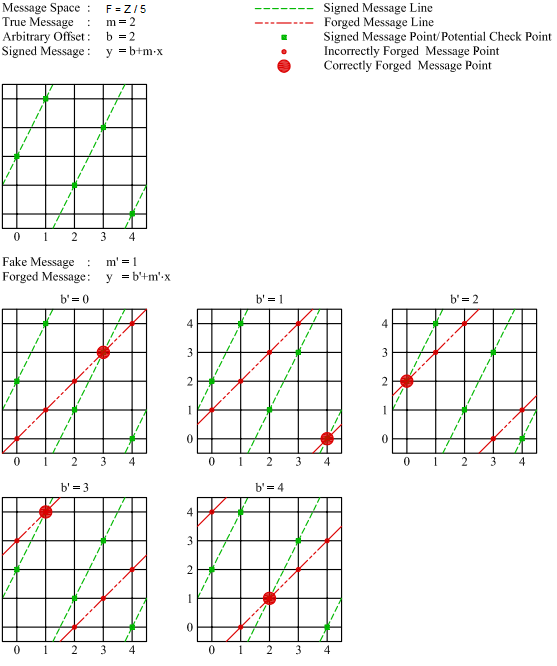
\includegraphics[width=\textwidth]{../../Graphics/PointAndLineExample.png}
\caption{Given a signed message ($m=2, b=2$) and a desired fake message ($m'=1$), each possible forged offset ($b'$) matches only one of the possible verifiers. Since the verifier is chosen at random, the chance of successful forging is $\frac{1}{p}$.}
\label{img:ForgingVerifiableMessageForUnbounded}
\end{figure}

\subsection{Overview}

Like SBP, SUIP is based on a sequence of ``fake" rounds followed by a definitive round. But SUIP's round messages are all specified in advance by the dealer. Each player has a list of messages to send, one per round. A message is composed of a $t$ of $n$ share for the round secret, which is the true secret on the definitive round but random on other rounds, and $t$ of $n$ shares for several round indicators, which are 0 on the definitive round but random on other rounds. Players recognize the definitive round, and thus learn the secret is the round secret, by noticing when all of the round indicators are 0.

SUIP can terminate in two ways, based on the lengths of the lists of messages and the definite round. Either the definitive round will occur before any of the players run out of messages to send, hereafter referred to as the ``normal case'', or it will occur on the round after a single player has run out of messages to send, hereafter referred to as the ``short case". The player who runs out of messages in the short case is called the short player. The dealer gives a ``short message'' to all players that contains the short player's missing message. The short message's contents are masked adding them to the short player's last message to send, to ensure it can't be used when the short player is not participating.

All messages, except the short message, are verified using the scheme explained in Section \ref{sec:vermes}. Every player has verifiers for every message they expect to receive. Every player has signatures for every receiver for every message they expect to send. The short message is verified implicitely by the round indicators: when it is applied in the wrong round or to the wrong player it effectively randomizes the round indicators, meaning the probability they are all 0 can be made as small as necessary.

Each round every player broadcasts their message for the round and verifies the messages they have received. If there are at least $t$ available round messages then the round secret and round indicators are easily recovered. If there are fewer than $t-1$ available round messages then the round secret and round indicators can't be recovered and the protocol aborts. If there are exactly $t-1$ available round messages then the short case may be occuring and players will attempt to use the short message to recover a $t$'th round message. For each player who did not send a valid message this round, but was cooperating until now, a potential round message is created by adding the short message's contents to the player's previous message's contents. If none of the potential short messages results in the round indicators all being 0, then the short case is not occuring and there are only $t-1$ players remaining so the protocol aborts.

See Algorithms \ref{alg:SUIP:Dealer} and \ref{alg:SUIP:Player} and Figure \ref{Ex:SUIP} for more details.

\begin{algorithm}
  \caption{Dealer Protocol for SUIP}
  \label{alg:SUIP:Dealer}
  \begin{algorithmic}[1]
    \INPUT Finite field $\mathbb{F}$
    \INPUT Total number of shares $n$ and threshold $t$
    \INPUT Marginal probability of definitive round occuring $\alpha$
    \INPUT Minimum message list size $\beta$
    \INPUT Message list marginal termination probability $\gamma$ satisfying $\gamma \leq \alpha$
    \INPUT Secret value $s$ from $\mathbb{F}$
    \OUTPUT Ordered list of $n$ shares
    \STATE Choose the minimum number of indicators as explained in Section \ref{Sec:SUIP:MinIndicators}
    \STATE Generate an ordered list $L$ of $n$ list lengths
    	$$D_i = Random(Geometric(stopChance: \gamma))$$
    	$$L_1 = \beta + D_1 \text{, } \text{ } \text{ } L_i = L_{i-1} + 1 + D_i$$
    \STATE Shuffle the list lengths, noting the new index $c$ of the shortest list
    \STATE Choose the definitive round $r$ as explained in Section \ref{Sec:SUIP:ChooseRound}
    \STATE Generate Shamir shares for the round secrets and indicators
    	$$S_{i} = CreateShamir(if(i = r, s, Random(\mathbb{F})), \mathbb{F}, n, t) \text{ for } i \in [1, L_n+1]$$
    	$$I_{i,j} = CreateShamir(if(i = r, 0, Random(\mathbb{F})), \mathbb{F}, n, t) \text{ for } i \in [1, L_n+1], j \in [1, \omega]$$
    \STATE Create signatures and verifiers for every share for every sending and receiving player
    \STATE Compute the short message $X$ composed of the short secret $X_0$ and short indicators $X_{1..\omega}$
    	$$X_0 = S_{r,c} - S_{r-1,c} \text{, } \text{ } \text{ } XI_j = I_{r,j,c} - I_{r-1,j,c} \text{ for } j \in [1, \omega]$$
    \STATE Return the ordered list $R$ of $n$ shares $R_i$
    	$$R_i = (i, X, S_{i,j}, I_{i,k,j}, VerifiersUpToRound(L_i+1), SignaturesUpToRound(L_i))$$
    	$$\text{for } i \in [1, n], j \in [1, L_i], k \in [1, \omega]$$
  \end{algorithmic}
\end{algorithm}

\begin{algorithm}
  \caption{Player Protocol for SUIP}
  \label{alg:SUIP:Player}
  \begin{algorithmic}[1]
    \INPUT Finite field $\mathbb{F}$
    \INPUT Total number of shares $n$ and threshold $t$
    \INPUT Share index $i$
    \INPUT Upper bound $r_{ceil}$ on the number of rounds
    \INPUT List of $r_{ceil}-1$ signed secret shares $S$ and arrays of signed indicator shares $I$
    \INPUT List $V$ of $r_{ceil}$ verifiers for other players' secret shares and indicators
    \INPUT Short message $X$
    \OUTPUT Success with secret $s$ or failure
    \STATE Mark all players, identified by indexes in $[1, n]$, including ourselves, as cooperating
    \STATE Let $r = 1$
    \WHILE { true }
      \STATE If the number of cooperating players is less than $t$ then exit with failure
      \STATE If $r < r_{ceil}$ then broadcast our round message $S_r, I_r$ to all players, including ourselves
      \STATE Receive round messages, that match corresponding verifiers in $V_r$, from cooperators
      \STATE Mark any player that did not send a verified round message as non-cooperating
      \STATE Let $N$ be the set of non-cooperating players who were cooperating last round
      \STATE Let $n_{msg}$ be the number of received round messages, counting ours if we sent one
      \STATE If $n_{msg} < t - 1$ then exit with failure
      \STATE Compute possible extra share sets, if necessary, by applying the short message to $N$
      		$$PossibleExtraSets = if(n_{msg} \geq t, \{\emptyset\}, \{\{LastMessage(e) + X\} | e \in N\}))$$
      \FOR {each $extra$ in $PossibleExtraSets$}
        \STATE Compute the round secret $s$ and indicators from received and $extra$ shares
        \STATE If all round indicators are 0 then exit with secret $s$
      \ENDFOR
    \ENDWHILE
  \end{algorithmic}
\end{algorithm}

\begin{figure}
  \caption{Example Dealer Run of SUIP}
  \label{Ex:SUIP}
  \begin{itemize}
    \item Finite Field $\mathbb{F}$ is integers mod 5
    \item Share count is $n = 2$ and threshold is $t = 2$
    \item Marginal round termination probability is $\alpha = \frac{1}{2}$
    \item Minimum list size is $\beta = 1$ and marginal termination probability is $\gamma = \frac{1}{3}$
    \item Number of indicators is $\omega = 1$
    \item Secret is $s = 3$
    \item Generate list lengths $L_1 = 4, L_2 = 3$ and final round $r = 3$
    \item Generate $MaxLength+1$ shamir shares for potential secrets and indicators
  
      \begin{tabular}{|r|r|r|r|r|}
      \hline
        Round & Potential Secret & Secret Shares & Indicator & Indicator Shares \\
      \hline
        1 & 2  & (1,2), (2,2) & 1 & (1,2), (2,3) \\
      \hline
        2 & 1  & (1,0), (2,4) & 1 & (1,1), (2,1) \\
      \hline
        \emph{3} & \emph{3}  & \emph{(1,4), (2,0)} & \emph{0} & \emph{(1,2), (2,4)} \\
      \hline
        4 & 1  & (1,4), (2,4) & 4 & (1,3), (2,2) \\
      \hline
        5 & 1  & (1,4), (2,4) & 4 & (1,3), (2,2) \\
      \hline
      \end{tabular}
      
    \item Generate verification information for every sender/receiver/share triplet
    \subitem In round 1 the secret share for index 1 is 2, and there is only one receiver. An arbitrary line with slope 2 is 1+2x. An arbitrary point on that line is (1,3). So for this message, share 1 could include the line offset 1 and share 2 could include the check point (1,3).
    \subitem Verification information is omitted from this example for brevity.
    
    \item Trim shares' list of messages to the corresponding list lengths $L_1 = 4, L_2 = 3$
    \item Compute the short message (although it won't be used)
    \subitem $X_0 = 4 - 0 = 4$, $X_1 = 2 - 4 = 3$
    \subitem Will not be used because the definitive round occurs before it is needed
    \item Resulting shares
    
      \begin{tabular}{|r|r|r|r|}
      \hline
        Index & Secret Shares & Indicator Shares & Signatures/Verifiers per receiver/sender \\
      \hline
        1 & 2, 0, 4, 4 & (2), (1), (2), (3) & \ldots, \ldots, \ldots, \ldots\\
      \hline
        2 & 2, 4, 0 & (3), (1), (4) & \ldots, \ldots, \ldots\\
      \hline
        short & 0 & (1) & -\\
      \hline
      \end{tabular}
  \end{itemize}
\end{figure}

\subsection{Analysis}

Let the finite field be $\mathbb{F}$, the number of players be $n$, the threshold be $t$, the marginal definitive round probability be $\alpha$, the marginal list termination probability be $\gamma$, the minimum list length be $\beta$, and number of indicators $\omega$. The expected number of rounds is $\frac{1}{\alpha}$. The expected size of the shortest list of messages is $\beta + \frac{1}{\gamma}$. The expected size of the largest list of messages is $\beta + \frac{n}{\gamma}$. The expected size of shares is $O((\beta + \frac{n}{\gamma}) \times n \times (log |\mathbb{F}|) \times \omega)$. The expected runtime of the dealer is $O((\beta + \frac{n}{\gamma}) \times n^2 \times (log |\mathbb{F}|) \times \omega \times Shamir(n, t))$. The expected runtime of the players is $O(\frac{1}{\alpha} \times n \times (log |\mathbb{F}|) \times \omega \times Shamir(n, t))$.

Because it is designed for potentially unbounded players, SUIP is expensive compared to its bounded variant SBP. SUIP's share size scales with the expected number of rounds, players, and indicators. By comparison, SBP has shares with size $O(n)$ and, unlike in SUIP, most of the information in the shares is not private. The dealer costs in SUIP also scale poorly, because the dealer effectively simulates every player's interaction with every other player for every round, whereas in SBP the dealer can handle each player individually and can ignore non-definitive rounds.

Given any probability $p < 1$, we can choose values for $\omega$, $\alpha$, $\beta$, and $\gamma$ that ensure running SUIP with at least $t$ rational players results in all rational players learning the secret with probability greater than $p$. $\beta$ must be large enough and $\gamma$ must be small enough to ensure the chance of cases where players can misbehave (all related to the short case) is sufficiently small (these cases are covered in Lemmas \ref{Lem:SUIP:ShortPlayerCoalitionsPremptivelyKnowShortRound}, \ref{Lem:SUIP:MaxSizeCoalitionsPremptivelyKnowShortRound}, \ref{Lem:SUIP:MinimumThresholdAndShortCaseMeansNoOneLearnsSecret}, \ref{Lem:SUIP:ShortPlayerMayLearnSecretExclusively}, \ref{Lem:SUIP:AllCoalitionsTempted}, and \ref{Lem:SUIP:MaxSizeCoalitionsTemptedMore}. Their effect is bounded by Lemmas \ref{Lem:SUIP:NoPlayerLearningSecretIsReducible}, \ref{Lem:SUIP:ShortPlayerLearningSecretExclusivelyIsReducible}, and \ref{Lem:SUIP:HighTemptationAvoidable}.). $\alpha$ must be small enough to ensure rational coalitions cooperate in the sufficiently likely case that they experience constant temptation $\alpha$. $\omega$ must be large enough to ensure the chance of malicious players affecting the other players is sufficiently small (see Lemma \ref{Lem:SUIP:MaliciousImmune}).

\begin{lemma} By choosing a large enough $\omega$, SUIP is immune to malicious coalitions \label{Lem:SUIP:MaliciousImmune} \end{lemma}
\begin{proof}
Malicious players will defect before or during the definitive round, because otherwise the other players will have more definitive round shares and will be more likely to learn the secret. In SUIP players defect by sending no round message or by sending a fake round message.

If a player sends no round message then they are marked as non-cooperating by all cooperating players (see Algorithm \ref{alg:SUIP:Player}). If a player sends a fake message then they are detected, with arbitrarily high probability bounded by the verification scheme, and marked non-cooperating by all cooperating players. Coalitions have multiple chances to send a fake message, but the probability of all the fake messages being detected is still arbitrarily high.

A player that has been marked non-cooperating by all cooperating players is effectively absent from the protocol, except the short message may be applied to them. They are sent no messages and the messages they send are discarded. Assuming applying the short message doesn't succeed, the protocol will terminate as if it had started without the non-cooperating players being present because rounds don't depend on information from non-cooperating players in previous rounds.

The probability of the short message being misapplied can be made arbitralily low by choosing a large enough $\omega$ as explained in Section \ref{Sec:SUIP:MinIndicators}. Therefore defectors are detected with arbitrarily high probability and applying the short message to them will not result in players learning the wrong secret with arbitrarily high probability. Therefore malicious players' effect on the protocol is equivalent to the effect of absent players.
\end{proof}

\begin{lemma} The short case occurs with probability $(1-\alpha)^\beta \times \frac{\gamma}{\alpha}$ \label{Lem:SUIP:ChanceOfShortCase} \end{lemma}
\begin{proof}
In order to reach the short case the protocol must have enough rounds to exceed the minimum list length. This occurs with probability $(1-\alpha)^\beta$. After the minimum list length is exceeded the probability of the definitive round being a short case is its marginal probability over the marginal probability of the definitive round, which is $\frac{\gamma}{\alpha}$. The probability of the short case occuring is their product.
\end{proof}

\begin{lemma} In the short case, coalitions containing the short player can pre-emptively detect the definitive round \label{Lem:SUIP:ShortPlayerCoalitionsPremptivelyKnowShortRound} \end{lemma}
\begin{proof}
If player has no messages to send in the coming round then they know that the short case is occuring, that they are the short player and that the coming round must be the definitive round. When a coalition contains the short player they pre-emptively detect the definitive round in the short case.
\end{proof}

\begin{lemma} In the short case, coalitions of size $t-1$, or individual players when $t = 2$, can pre-emptively detect the definitive round \label{Lem:SUIP:MaxSizeCoalitionsPremptivelyKnowShortRound} \end{lemma}
\begin{proof}
Let $C$ be a set of $t-1$ colluding players. Let $d$ be the short player. Let $r$ be the definitive round, occuring after $d$'s list of messages is exhausted.

Either $d \in C$ or $d \notin C$.

If $d \in C$ then the coalition can pre-emptively detect the definitive round by Lemma \ref{Lem:SUIP:ShortPlayerCoalitionsPremptivelyKnowShortRound}.

If $d \notin C$ then, after round $r-1$, the members of $C$ have enough round messages to determine if the short message will apply if any of the players outside of $C$ defect. When the short case occurs, they will be able to pre-emptively apply the short message to $d$, learn the secret, and defect.

Therefore a set of $t-1$ colluding players can pre-emptively detect the definitive round even when they do not include the short player.
\end{proof}

\begin{lemma} When $t=2$, no one learns the secret in the short case. \label{Lem:SUIP:MinimumThresholdAndShortCaseMeansNoOneLearnsSecret} \end{lemma}
\begin{proof}
When $t=2$ all players will pre-emptively detect the definitive round in the short case, by Lemma \ref{Lem:SUIP:MaxSizeCoalitionsPremptivelyKnowShortRound}, and want to defect.

All players who are not the short player will be able to defect on the definitive round. The short player is unable to defect on the definitive round, because the protocol doesn't place any constraints on their actions. But, because the short player knows all other players will defect on the round after the short player's list runs out, the short player has no incentive to cooperate on the preceeding round. Thus the short player will defect one round before the short case's definitive round.

Thus all players defect before or during the definitive round, meaning no definitive round messages are broadcast and therefore no player learns the secret.
\end{proof}

\begin{lemma} By choosing a large enough $\beta$, the probability of all players not learning the secret when $t=2$ can be made arbitrarily small. \label{Lem:SUIP:NoPlayerLearningSecretIsReducible} \end{lemma} 
\begin{proof}
As explained in Lemma \ref{Lem:SUIP:MinimumThresholdAndShortCaseMeansNoOneLearnsSecret}, all players may not learn the secret in the short case. But by Lemma \ref{Lem:SUIP:ChanceOfShortCase} the short case has probability that decreases exponentially as $\beta$ increases. Thus we can make the probability of all players not learning the secret arbitrarily small by increasing $\beta$.
\end{proof}

\begin{lemma} When $t=2$, the short player may learn the secret exclusively. \label{Lem:SUIP:ShortPlayerMayLearnSecretExclusively} \end{lemma} 
\begin{proof}
As explained in Lemma \ref{Lem:SUIP:MinimumThresholdAndShortCaseMeansNoOneLearnsSecret}, the short player will defect one round before the definitive round would occur due to the short case. When this round happens to be the definitive round in the normal case and there are 2 remaining rational players, one of which is the short player, the short player will unilaterally defect and learn the secret exclusively.
\end{proof}

\begin{lemma} By choosing a large enough $\beta$, the probability of short player learning the secret exclusively when $t=2$ can be made arbitrarily small. \label{Lem:SUIP:ShortPlayerLearningSecretExclusivelyIsReducible} \end{lemma} 
\begin{proof}
As explained in Lemma \ref{Lem:SUIP:MinimumThresholdAndShortCaseMeansNoOneLearnsSecret}, the short player will defect on the round before they know the short case would occur due to their list running out. In order for the short player to learn the secret exclusively, the round they defect on must be the definitive round due to the normal case. The probability of that occuring is the probability that the protocol ends in the normal case but would have ended in the short case if there had been another round.

If the shortest list has the minimum length $\beta$ then the probability is $(1-\alpha)^{\beta-1} \times \alpha \times \gamma$. If the shortest list does not have minimum length then the probability is $(1-\alpha)^\beta \times (1 - \frac{\gamma}{\alpha}) \times \gamma)$. Together they give an upper bound on the probability of the short player exclusively learning the secret:

$$(1-\alpha)^{\beta-1} \times (\alpha + (1-\alpha) \times (1 - \frac{\gamma}{\alpha})) \times \gamma$$

Since this upper bound decreases exponentially as $\beta$ increases, we can practically make the probability of the short player exclusively learning the secret arbitrarily small by increasing $\beta$.
\end{proof}

\begin{lemma} When $t > 2$, for non-colluding rational players, SUIP has constant temptation $\alpha$ \label{Lem:SUIP:NonColludersNotTemptedExceptT2} \end{lemma}
\begin{proof}
Each round has a marginal probability $\alpha$ of being the definitive round. Individual rational players can't determine if a round is the definitive round in the normal case until it has finished. They also can't detect the definitive round in the short case unless they are the short player or $t=2$, in which case they can't defect because the protocol places no constraint on their actions.

Therefore, when $t > 2$, non-colluding rational players either can't defect or believe they will learn the secret with probability $\alpha$ if they defect.
\end{proof}

\begin{lemma} For rational coalitions $C$ up to size $t-2$, SUIP has worst deal maximum temptation $1$ and expected deal maximum temptation $\alpha + (1-\alpha)^{\beta+1} \times \frac{\gamma}{\alpha} \times \frac{|C|}{n}$ \label{Lem:SUIP:AllCoalitionsTempted} \end{lemma}
\begin{proof}
If a coalition contains the short player then and the short case occurs they, by Lemma \ref{Lem:SUIP:ShortPlayerCoalitionsPremptivelyKnowShortRound}, they will pre-emptively detect the definitive round. This will allow them to defect and not affect their chances of learning the secret. They encounter a temptation of $1$. If the short player is outside the coalition or the normal case occurs, then the coalition experiences a constant temptation of $\alpha$.

The dealer assigns the short message to a random player when generating the shares. The probability of a coalition $C$ containing the short player is $\frac{|C|}{n}$. The probability of the short case is $p_{short} = (1-\alpha)^\beta \times \frac{\gamma}{\alpha}$. The worst deal maximum temptation, based on the short case occuring and the short player being in the coalition, is $1$. The expected deal maximum temptation is $1 \times p_{short} \times \frac{|C|}{n} + \alpha \times (1 - p_{short} \times \frac{|C|}{n})$, which expands and re-arranges to $\alpha + (1-\alpha)^{\beta+1} \times \frac{\gamma}{\alpha} \times \frac{|C|}{n}$.
\end{proof}

\begin{lemma} For rational coalitions of size $t-1$, or individual players when $t=2$, SUIP has worst deal maximum temptation $1$ and expected deal maximum temptation $\alpha + (1-\alpha)^{\beta+1} \times \frac{\gamma}{\alpha}$ when $t > 2$ \label{Lem:SUIP:MaxSizeCoalitionsTemptedMore} \end{lemma}
\begin{proof}
By Lemma \ref{Lem:SUIP:MaxSizeCoalitionsPremptivelyKnowShortRound}, coalitions of size $t-1$ can pre-emptively detect the definitive round in the short case. In that case they can defect and still be guaranteeed to learn the secret. The short case is a possible deal, so the worst deal maximum temptation is $1$.

A deal that causes the short case has a maximum temptations of $1$ for the coalition. Otherwise the coalition experiences a constant temptation of $\alpha$. The expected maximum temptation of a deal is the maximum temptation of both cases weighted by their likelihood, which is $1 \times p_{short} + \alpha \times (1-p_{short})$ which expands and re-arranges into $\alpha + (1-\alpha)^{\beta+1} \times \frac{\gamma}{\alpha}$.
\end{proof}

\begin{lemma} By choosing a large enough $\beta$, the probability of a deal of SUIP having constant temptation $\alpha$ can be made arbitrarily high \label{Lem:SUIP:HighTemptationAvoidable} \end{lemma}
\begin{proof}
The cases were rational players or coalitions can pre-emptively detect SUIP's definitive round are all contained to the short case. In the normal case players always believe the next round is the definitive round with probability $\alpha$.

By Lemma \ref{Lem:SUIP:ChanceOfShortCase}, the probability of the short case occuring is $(1-\alpha)^\beta \times \frac{\gamma}{\alpha}$. Since this probability decreases exponentially as $\beta$ increases, we can practically make the probability of the short case arbitrarily small. Thereffore we can make the probability of SUIP not having constant temptation $\alpha$ arbitrarily small by increasing $\beta$.
\end{proof}

\subsection{Choosing a definitive round with the proper distribution}
\label{Sec:SUIP:ChooseRound}

Every round must have a marginal probability $\alpha$ of being the definitive round. But once we exceed round $\beta$ there are two ways to terminate: the normal way or due to the shortest list ending. The shortest list has a marginal probability $\gamma$ of terminating and we want an overall $\alpha$ marginal probability of termination. The marginal termination probability for the normal case $x$ should satisfy $\gamma + x \times (1 - \gamma) = \alpha$. Solving for $x$ gives $x = \frac{\alpha - \gamma}{1 - \gamma}$.

Algorithm \ref{alg:SUIP:DefinitiveRound} details how to choose a definitive round $r$ with an overall geometric distribution, given that we have already generated a random shortest list length $L_c = \beta + RandomGeometric(\gamma)$ and we must satisfy $r < L_c$.

\begin{algorithm}
  \caption{Choosing SUIP's Definitive Round}
  \label{alg:SUIP:DefinitiveRound}
  \begin{algorithmic}[1]
    \INPUT The marginal definitive round probability $\alpha$ 
    \INPUT The minimum possible list length $\beta$
    \INPUT The marginal end of list probability $\gamma$ satisfying $\gamma < \alpha$
    \INPUT Length $L_c$ of the shortest list of messages
    \OUTPUT The definitive round $r$
    \STATE Let $r = 1$
    \WHILE { $r \leq \beta$ }
      \STATE Let $b$ be true with probability $\alpha$
      \STATE If $b$ is true then Return $r$
      \STATE Increment $r$ by 1 
    \ENDWHILE
    \WHILE { $r \leq L_c$ }
      \STATE Let $b$ be true with probability $\frac{\alpha - \gamma}{1 - \gamma}$
      \STATE If $b$ is true then Return $r$
      \STATE Increment $r$ by 1
    \ENDWHILE
    \STATE Return $r$
  \end{algorithmic}
\end{algorithm}

\subsection{Choosing a Large Enough Number of Indicators $\omega$}
\label{Sec:SUIP:MinIndicators}

When the short message is applied to the wrong player or in the wrong round, the resulting indicators are effectively random. If they happen to all be 0 then players will accept the wrong secret instead of aborting the protocol. Because malicious coalitions of unbounded players can find these cases, we need to bound the probability of any existing.

Suppose our goal is to ensure the probability is less than $\frac{1}{c}$ for some value $c$. There is a $\frac{1}{|\mathbb{F}|^\omega}$ chance of $\omega$ indicators coming up 0. If there are $r$ rounds, $n$ players, and the threshold is $t$ then there are $\binom{n}{t} \times t \times r$ ways the short message can be applied. The probability of a bad case existing is thus $\frac{\binom{n}{t} \times t \times r}{|\mathbb{F}|^\omega}$. Solving $\frac{\binom{n}{t} \times t \times r}{|\mathbb{F}|^\omega} < \frac{1}{c}$ for $\omega$ gives $\omega > log_{|\mathbb{F}|} (\binom{n}{t} \times t \times r \times c) = (log_{|\mathbb{F}|} c) + (log_{|\mathbb{F}|} r) + log_{|\mathbb{F}|} (\binom{n}{t} \times t)$.

Our bound for $\omega$ depends on the number of rounds $r$, but this is not ideal since it may ``leak" information about $r$ to the players via $\omega$. Since $r$ is a random variable, we can spend some of our probability bound choosing a high enough cutoff value $r'$. If we choose to allocate a $\frac{1}{c \times 2}$ probability to not exceeding the cutoff and the remaining $\frac{1}{c \times 2}$ probability to ensuring there are no bad cases when we don't exceed the cutoff, then we meet the overall bound of $\frac{1}{c}$. We solve for the cutoff round $r'$ using the fact that $r$ follows a geometric distribution parameterized by $\alpha$: $(1 - \alpha)^{r'-1} \leq \frac{1}{2 \times c}$, which solves to $r' \geq 1 + log_{\frac{1}{1-\alpha}}(2 \times c)$. We get our final bound by updating our previous $r$-dependent bound, feeding in a maximum probability of $\frac{1}{2 \times c}$ and the minimum value of $r'$:

$$\omega > (log_{|\mathbb{F}|} (2 \times c)) + (log_{|\mathbb{F}|} (1 + log_{\frac{1}{1-\alpha}}(2 \times c))) + log_{|\mathbb{F}|} (\binom{n}{t} \times t)$$

For practical cases ($|F| \geq 2^{256}, n \leq 200, \alpha \geq \frac{1}{100}, c \leq 2^{256}$) a large enough value of $\omega$ is 2. For theoretical cases, the minimum number of indicators grows logarithmically against the magnitude or inverse magnitude of the protocol's parameters and $c$. Therefore we can practically achieve an arbitrarily high probability of the short message not being abusable.

\subsection{Consequences of the Short Case}

The primary complicating factor in running and analyzing SUIP is the existence of the short case. In particular, it is the reason the protocol must have some probability of failing in the presence of rational players who want to cooperate until they learn the secret. A protocol with a short case can't be immune to rational coalitions.

All protocols based around the dealer giving players lists of messages to send will have an equivalent to the short case. This is a consequence of the players using the length of the lists to derive a maximum value for the definitive round. The protocol must sometimes lasts until a round where a player knows it is the definitive round and then that player will want to defect. The protocol has a short case.

Removing the short case from a protocol is not trivial. For example, if you attempt to eliminate the short case by having the dealer recreate shares if it occurs, players will use that knowledge to get better bounds on the maximum value of the definitive round and a new type of short case will be created as a result.

Players need an unbounded amount of entropy when opponents may be unbounded and that entropy must either come from the dealer or the players. It is convenient, and perhaps necessary, for the entropy to come from the dealer in order to allow for verification. But when the entropy comes from the dealer the protocol must have a short case. Whether or not entropy generated by the players can be properly verified, although this is an avenue for future work.

The short case has particularly high costs for the $t=n=2$ case. Every 2-of-2 protocol with a short case must choose between everyone learning the secret in the short case or not learning the wrong secret when the other player is malicious. SUIP prevents a malicious player from convincing the other player to accept the wrong secret. Kohl and Noar's 2-of-2 protocol \cite{kol08} guarantees two rational players will both learn the secret. The trade-off is a consequence of deciding whether or not, when a player appears to defect, the remaining player can check if the short case is occuring. If the remaining player can check for the short case then they can do so before the definitive round starts, learn the secret, stop participating, and thus prevent the short player from learning the secret. If the remaining player can't check for the short case then they can't distinguish between the short case occuring and a malicious player defecting on a non-definitive round.

\subsection{Summary}

SUIP is immune to malicious coalitions, but not immune to rational coalitions. SUIP succeeds probabilistically, even if all players are rational, based on whether or not the dealer generates shares containing the short case. When the short case occurs, and there are coalitions or $t=2$, some players may not learn the secret.

We anticipate future work to focus on eliminating the short case or reducing its effects. If the short case can't be eliminated then we conjecture that no protocol for unbounded players achieves immunity against rational coalitions.





\chapter{Asynchronous Broadcast}

In practice, communication is not synchronous. The internet is asynchronous and unreliable in nature, requiring protocols allowing for those possibilities. This chapter presents protocols that work when we assume Asynchronous Broadcast instead of Synchronous Broadcast.

Unlike synchronosu broadcast, asynchronous broadcast does not allow senders to synchronize their sends. Rational players, who have an incentive to wait to receive messages before sending, will tend to deadlock unless the protocol specifies a message ordering.

Asynchronous broadcast still assumes reliability, timeliness, and consistency across receivers. If a sender chooses to send a message then all receivers will receive the same message in bounded time. If a sender chooses to send no message, then all receivers will know, in bounded time, no message was sent.

\section{Limitations of all Asynchronous Protocols}

\begin{lemma} If all players are rational, the secret is conspicuous, and communication is asynchronous then at least one player will not learn the secret \label{Lem:Async:ConspicuousMustSacrifice} \end{lemma}
\begin{proof}
We will prove this result by contradiction. Assume all players learn the secret.

Let $r$ be the first round such that, at the end of round $r$, all players know the secret. Let $L$ be the set of players who learn the secret during round $r$. Let $s$ be the expected sender of round $r$'s message. Let $m$ be the message, or lack of a message, sent in round $r$.

$m$ is a message, not the lack of a message. Because the secret is conspicous, players can attempt to brute force it by pre-emptively trying likely messages. The easiest possibility to try is the lack of a message. If $m$ was the lack of a message, then the memberes of $L$ would have tried this possibility at the end of the previous round and learned the secret before round $r$. If $m$ is the lack of a message then $r$ is not the first round a player learns the secret, contradicting our assumptions.

$s \in L$. If $s$ knew the secret before round $r$, then $s$ would have sent no message. A rational player who knows the secret only cares about preventing or delaying others from learning the secret. Sending the correct message can only help others learn the secret whereas, because the secret is conspicuous, sending nothing (or an invalid message) can't hurt. Therefore, because $s$ did not know the secret before round $r$ but all players know the secret at the end of round $r$, $s$ must have learned the secret during round $r$.

$s \notin L$. Because $s$ received no information during round $r$ (since there were no other senders), $s$ can't have learned any new values. So $s$ did not learn the secret during round $r$.

Contradiction: $s \in L$ and $s \notin L$.

The assumption that all players learned the secret is false.

At least one player did not learn the secret.
\end{proof}

All rational asynchronous protocols for conspicuous secrets must use a sacrificial player. This is a consequence of the fact that a player can check if they have or do not have a conspicuous secret. When the secret is inconspicuous it is possible for a player to have a value and be unsure if it is the secret or not. This allows the player to be incentivized into cooperating for a longer amount of time, and replaces the need for a sacrifical player.

\begin{lemma} If all players are rational and communication is asynchronous then rational coalitions have a greater than $\epsilon > 0$ chance of pre-emptively learning the secret \label{Lem:Async:CoalitionsMayPreempt} \end{lemma}

A coalition pre-emptively learns the secret when members of the coalition learn the secret before any player would have if there were no collusion occuring.

\begin{proof}
Let $n$ be the number of players.
Let $C$ be a rational coalition of players, selected randomly, with size less than the threshold $t$.
Let $r$ be the first round where a player would learn the secret if there were no collusion.
Let $L$ be the set of learners: players who learn the secret in round $r$.
Let $s$ be the sender of round $r$'s message.

The sender can not be one of the learners because the sender is receiving no new information during round $r$.

If the sender and at least one of the learners are in the coalition, then the coalition can internally simulate sending round $r$'s message before round $r$ occurs and thereby pre-emptively learn the secret. The probability of this occuring is $\frac{|C|}{n} \times \frac{\binom{n - |C|}{|L|}}{\binom{n - 1}{|L|}}$. This function varies with $L$, which the protocol has some control over. Higher values of $L$ give higher probabilities, so a lower bound for any protocol is setting $L$ to its minimum value: 1. This gives a lower bound probability of $\frac{|C| \times (|C| - 1)}{n \times (n-1)}$, which is independent of the protocol.
\end{proof}

Pre-emptively learning the secret allows a coalition to defect earlier, potentially depriving other players of shares and causing them to not learn the secret. All rational asynchronous protocols are vulnerable to coalitions pre-sharing their messages internally. Every protocol has a lower bound of at least a $\frac{|C| \times (|C| - 1)}{n \times (n-1)}$ chance of coalitions pre-emptively learning the secret. This minimum lower bound can probably be improved.

We conjecture that, as a result of Lemma \ref{Lem:Async:CoalitionsMayPreempt}, all asynchronous broadcoast protocols are either not immune to rational coalitions or not immune to malicious coalitions.


\section{Asynchronous Protocol for Conspicuous Secrets and Bounded Opponents}

The asynchronous protocol for inconspicuous secrets relied on the secret's inconspicuousness to allow the final $t-1$ senders to learn the secret. Even though they knew the most likely secret, they couldn't check it. When the secret is conspicuous, we can't rely on this property and must sacrifice one of the players.

\subsection{Overview}

This protocol is derived from the synchronous bounded protocol. The main difference is that the target round occurs at different times for different players, staggering their completion.
 
The proposed algorithm is basically a generalization of the synchronous algorithm. The main differences are that every player gets a different set of underlying secret shares to reveal, and they receive those shares on different rounds. Staggering the target rounds allows more players to stay in the dark about the game finishing until they have sent their message.

\begin{figure}
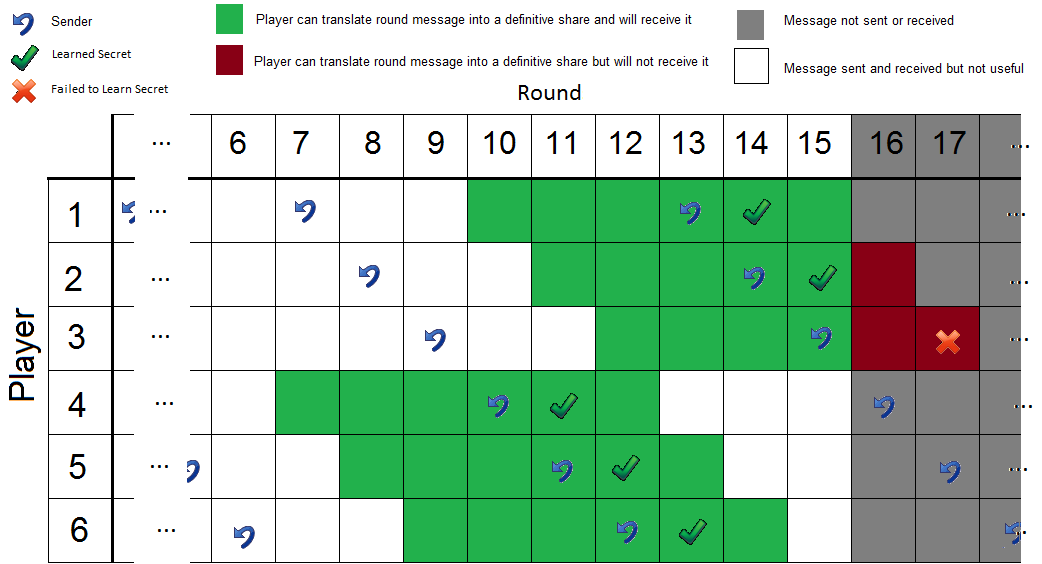
\includegraphics[width=\textwidth]{../../Graphics/AsyncVerifiedSecret_n6t5d1.png}
\caption{Example run of asynchronous conspicuous bounded protocol with parameters $n=6, t=5, \delta=1$. A player is sacrificed.}
\label{AsyncExample1}
\end{figure}

\begin{algorithm}
  \caption{Dealer Protocol}
  \label{alg:ABC_Dealer}
  \begin{algorithmic}
    \INPUT A large prime $p$ defining the size of the finite field containing the secret
    \INPUT The number of shares $n$ and threshold $t$
    \INPUT The share shortage $\delta$ satisfying $0 < \delta < t$
    \INPUT The marginal probability of termination $\alpha$
    \INPUT The verifiable random function scheme $VRF$
    \INPUT The commitment scheme $CS$
    \INPUT The secret $s$
    \OUTPUT $n$ shares with threshold $t$ of the secret $s$
    \STATE Create a commitment $c$ to the secret $s$ in the commitment scheme $CS$
    \STATE Create $n$ verifiable functions defined by the key pairs $G_i, V_i = VRFS.CreateKeyPair()$
    \STATE Pick a target round $r$ from $GeometricDistribution(\alpha)$
    \FOR{For each share index $i$ from 1 to $n$}
      \STATE Generate a set $S$ of $n$ shamir shares with threshold $t$ for the secret $s$
      \STATE Compute the first unblinding round $r_{unblind} = r + (i-r \pmod{n})$
      \STATE Compute the share/message offsets $\mathbb{F}_j = VRFS.ValueOf(G_j, r_{unblind} + (j-r_{unblind} \pmod{n})) + S_j$
      \STATE Yield a share composed of public information $n, t, c, V$ and private information $i, G_i, \mathbb{F}$
    \ENDFOR
  \end{algorithmic}
\end{algorithm}
\begin{algorithm}
  \caption{Player Protocol}
  \label{alg:ABC_Player}
  \begin{algorithmic}
    \INPUT A large prime $p$ defining the size of the finite field containing the secret
    \INPUT The number of shares $n$ and threshold $t$
    \INPUT The commitment $c$ to the unknown secret
    \INPUT The list of all VRF public keys $V$
    \INPUT Our index $i$
    \INPUT Our VRF private key $G_i$
    \INPUT Our list of share/message offsets $\mathbb{F}$
    \OUTPUT Succeed with secret or Failure
    \STATE Mark all players as cooperating, including ourselves
    \STATE Let $Q$ be an empty queue
    \STATE Let $r = 1$
    \WHILE {not failed or succeeded}
	  \STATE Fail if fewer than $t$ players are marked as cooperating
	  \IF {$r = i \pmod{n}$} 
	  	 \STATE Let $s, b = VRFS.ValueAndProof(G_i, r)$ 
	  	 \STATE Send the message $s, b$
	  \ELSE
	     \STATE Let $e$ be the player with index $r \pmod{n}$
	     \STATE Let $s$, $b$ be the message value and proof received from $e$ (if any)
	     \STATE If $e$ sent no message or a message failing $VRFS.Check(V_{r \pmod{n}}, s, b)$ then mark $e$ as non-cooperating
	     \STATE If $e$ is marked as non-cooperating then skip to the next round
	   \ENDIF
	   \STATE Enqueue $s+F_{r \pmod{n}}$ in $Q$
       \STATE Remove the oldest item in $Q$ if it has more than $t$ items
	   \STATE Let the potential secret $s$ be the value at 0 of the polynomial interpolated from the points in $Q$
	   \STATE If $c$ matches $s$ then succeed with the secret $s$
       \STATE Increment $r$
	\ENDWHILE
  \end{algorithmic}
\end{algorithm}

\begin{lemma} Rational Coalitions with size greater than $\delta$ may learn the secret early enough for all of its members to defect. \end{lemma}

All of the members of a rational coalition can stop cooperating after any one of them learns the secret. The earlier the secret is learned, the more likely it is that many of the colluders can defect instead of cooperating on important rounds. We already know, from [lemma bla], that all asynchronous protocols allow rational coalitions to potentially learn the secret earlier than any of its members should be able to. But that does not imply the coalition learns the secret early enough to act on the information. This result is stronger, implying the coalition can learn the secret early enough for all of its members to defect before they otherwise would have. 

\begin{proof}
Assume all players outside of the coalition are cooperating.

On some round $r$ the first important share will be sent. The last important share is on round $r+n+t-1$ but, if all players are rational, only round $r+n+t-1-\delta$ will be reached. The first $t-\delta-1$ and final $\delta$ important shares to be sent are not important to their senders. The $n$ other important shares to be sent are important to their senders. On round $r+t-\delta$ the first share important to its sender is sent.

On round $r+t-1$, the sender for that round needs at least $\delta$ shares from future rounds before they will learn the secret. If the sender is colluding, they may already have access to those shares. In that case all members of the coalition will defect on round $r+t-\delta$. Since all players send one message between round $r+t-\delta$ and round $r+t-\delta+n-1$, which would be reached normally, every member of the coalition has managed to avoid sending at least one important message.

Coalitions with size greater than $\delta$ can have a sender on round $r+t-\delta$ and the remaining members may hold the $\delta$ future round shares the sender needs. This circumstance is sufficient, but by no means necessary, to show that some fraction of possible coalitions will learn the secret early enough for all of their members to defect.
\end{proof}

\begin{lemma} For Non-Colluding Rational Players, the protocol's Maximum Temptation is $0$ \end{lemma}
\begin{proof}
When a player sends for the final time, they need $\delta$ more shares before they can learn the secret. If they defect instead of sending, other players will stop sending them shares. Since they are not colluding and not being sent shares, they won't be able to access the shares they need. Therefore if they defect they will not learn the secret.
\end{proof}

This optimal maximum temptation is possible because some players are sacrificed. Instead of guaranteeing all cooperators learn the secret, we have guaranteed all defectors do not learn the secret.

\begin{lemma} If all players are rational and non-colluding then exactly $n - \delta$ players learn the secret \end{lemma}
\begin{proof}
When a player sends for the final time, they need $\delta$ more shares. The last player to send will not learn the secret, because they receive 0 more shares and $\delta > 0$. The before last player, who is not the same player because players take turns sending messages, will only learn the secret if $\delta = 1$. Similarly, the before before last player only learns the secret if $\delta \leq 2$. Extrapolating, we see that the $i$'th last sender only learns the secret if $i > \delta$. Therefore exactly the $\delta$ last senders, who are distinct because $\delta < n$, will not learn the secret.
\end{proof}

The value of $\delta$ is a trade-off between resistance against coalitions and the number of sacrificial players. A higher $\delta$ requires sacrificing more players. A lower $\delta$ increases the number of shares a player has when they send, meaning fewer colluders are needed to pre-emptively learn the secret.



\section{Asynchronous Protocol for Inconspicuous Secrets and Bounded Opponents}

ABCP, the asynchronous bounded conspicuous protocol presented in the previous section, sacrifices a player. In fact, sacrificing a player is a necessary property of all conspicuous asynchronous protocols, by Lemma \ref{Lem:Async:ConspicuousMustSacrifice}. This raises the obvious question: is an asynchronous protocol with no necessary sacrifices possible when the secret is not conspicuous? This section answers that question by presenting a protocol, hereafter referred to as ``ABIP'' (asynchronous bounded inconspicuous protocol), that does not require a player to be sacrificed.


\subsection{Overview}

ABIP is a modified version of SBP, except the commitment scheme is replaced by a lower threshold on the secret shares. The protocol is divided into a sequence of check rounds followed by a definitive round, during which players learn the secret. Each round is divided into turns where each player sends a message created by a verifiable random function (VRF). Players add messages to sender specific offsets to create round shares. Both the offsets and VRFs are chosen beforehand by the dealer. Before the definitive round the round shares are random but during the definitive round the round shares are the Y coordinates of Shamir shares, with a threshold of $t-1$, for the secret. This property is a consequence of how the offsets and VRFs are chosen by the dealer.

Players recognize the definitive round in two ways. The first method, which we call the ``threshold method", checks if $t$ round shares fit on a polynomial of degree $t-2$. This occurs only, with arbitrarily high probability, during the definitive round because a set of $t$ random points from a finite field $\mathbb{F}$ will, with probability $1 - \frac{1}{|\mathbb{F}|}$, not fit on a polynomial of degree $t-2$. The second method, called the ``recovery method'', is noticing that exactly $t-1$ round shares were broadcast in a round. The first $t-1$ senders of a round must use the recovery method because the other players can use the threshold method, learn the secret, and defect before they broadcast their own definitive round share.

See Algorithms \ref{alg:ABIP:Dealer} and \ref{alg:ABIP:Player} and Figure \ref{Ex:ABIP} for more details.

\begin{algorithm}
  \caption{Dealer Protocol for ABIP}
  \label{alg:ABIP:Dealer}
  \begin{algorithmic}
    \INPUT A finite field $\mathbb{F}$
    \INPUT Number of shares $n$ and threshold $t$
    \INPUT Marginal probability of termination $\alpha$
    \INPUT Verifiable random function scheme $VRF$
    \INPUT Secret $s$ in $\mathbb{F}$
    \OUTPUT $n$ shares
    \STATE Create $n$ VRFS key pairs, one for each player
    	$$G_i, V_i = VRFS.CreateKeyPair()$$
    \STATE Generate $n$ shamir shares, with a threshold of $t-1$, for the secret $s$
    	$$S_i = CreateShamir(s, n, t - 1, \mathbb{F})$$
    \STATE Pick a random round $r$ to be the definitive round
        $$r = Random(Geometric(\alpha))$$
    \STATE Compute ordered list $Y$ of $n$ offsets for each player
    	$$Y_i = S_i - VRFS.ValueOf(G_i, r)$$
    \STATE Return the ordered list $R$ of $n$ ABIP shares each containing an index, secret key, all public keys, and all offsets 
    	$$R_i = (i, G_i, V, Y)$$
  \end{algorithmic}
\end{algorithm}

\begin{algorithm}
  \caption{Player Protocol for ABIP}
  \label{alg:ABIP:Player}
  \begin{algorithmic}
    \INPUT A finite field $\mathbb{F}$
    \INPUT Number of shares $n$ and threshold $t$
    \INPUT Verifiable random function scheme $VRFS$
    \INPUT Share index $i$, generator $G_i$, all verifiers $V$, all offsets $Y$
    \OUTPUT Secret $s$ or Failure
    \STATE Mark all players, identified by indexes in $[1, n]$, including ourselves, as cooperating
    \STATE Let $r = 1$
    \WHILE { true }
      \STATE If fewer than $t$ players are marked as cooperating then Exit with Failure
      \STATE Let $S$ be an empty set of points in $\mathbb{F}^2$
      \STATE Let $P(S)$ evaluate to the polynomial created by interpolating the points in $S$
      \STATE Include the point $(i, VRFS.ValueOf(G_i, r) + Y_i)$ in $S$
      \FOR {$j$ = 1 to $n$}
        \STATE If $j = i$ then send the message $VRFS.ValueAndProof(G_i, r)$
        \STATE Let $a, p$ be the expected message from the player with index $j$
        \IF {$a, p$ was not received or does not satisfy $VRFS.Verify(V_j, a, p)$}
          \STATE Mark player $j$ as not cooperating
        \ELSE
          \STATE Include the point $(j, a + Y_j)$ in $S$
          \IF {$S$ has exactly $t$ points and $P(S)$ has degree less than $t-1$}
            \STATE Exit with the secret $s = P(S)(0)$
          \ENDIF
        \ENDIF
      \ENDFOR
      \IF {$S$ has exactly $t-1$ points}
        \STATE Exit with the secret $s = P(S)(0)$
      \ENDIF
      \STATE Increment $r$
    \ENDWHILE
  \end{algorithmic}
\end{algorithm}

\begin{figure}
  \caption{Example run of ABIP}
  \label{Ex:ABIP}
  \begin{itemize}
    \item Finite field $\mathbb{F}$ is integers mod 5
    \item Share count $n = 2$ and threshold $t = 2$
    \item Marginal definitive block probability $\alpha = \frac{1}{3}$
    \item Verifiable Random Functions $PedagogicalRSA(p: 7, q: 11)$
    \item Secret $s = 3$
    \item Create RSA key pairs for VRFS for each of the 2 players
    \subitem $V_1, G_1 = 17, 53$
    \subitem $V_2, G_2 = 13, 37$
    \item Pick the start of the definitive round $r = 3$
    \item Create the Shamir shares $S_i$ for each player based on a generated polynomial $P$
    \subitem $P(x) = 3 \pmod{5}$
    \subitem $S_1 = (1, 3)$, $S_2 = (2, 3)$
    \item Compute the offsets 
    \subitem $X_1 = 3 - (3^{53} \pmod{77}) \equiv 3 \pmod{5}$
    \subitem $X_2 = 3 - (3^{37} \pmod{77}) \equiv 2 \pmod{5}$
    \item Transition from dealer protocol to player protocol 
  \end{itemize}
  \begin{tabular}{|r|r|r|r|r|}
    \hline
    Round & Msg mod $77$   & Check mod $77$ & Round share mod $5$    & Combine mod $5$\\
    \hline
    1 & $M_1 = 1^{53} = 1$  & $1^{13} = 1$   & $P(1) = 1+3 = 4$  & $P_1(x) = 0 + 4x$\\
      & $M_2 = 1^{37} = 1$  &  $1^{17} = 1$  & $P(2) = 1+2 = 3$  & $deg(P_1) < 1$: False\\
    \hline
    2 & $M_1 = 2^{53} = 74$ & $74^{13} = 2$  & $P(1) = 74+3 = 2$ & $P_2(x) = 1 + x$\\
      & $M_2 = 2^{37} = 51$ &  $51^{17} = 2$ & $P(2) = 51+2 = 3$ & $deg(P_2) < 1$: False\\
    \hline
    3 & $M_1 = 3^{53} = 5$  & $5^{13} = 3$   & $P(1) = 5+3 = 3$  & $P_3(x) = 3$\\
      & $M_2 = 3^{37} = 31$ & not sent       & $P(2) = 31+2 = 3$ & $deg(P_3) < 1$: True\\
    \hline
  \end{tabular}
  \begin{itemize}
    \item Player 2 thresholds $deg(P_3) < 1$ by having $M_2$ and receiving $M_1$
    \item Player 1 recovers $deg(P_3) = 0$ when player 2 stops participating
    \item Both players have enough shares to solve $P_3$
    \item Both players learn the secret $s = P_3(0) = 3$  
  \end{itemize}
\end{figure}


\subsection{Analysis}

ABIP's performance is similar to SBP's, with identical asymptotic time and space costs. Let the number of players be $n$, the threshold be $t$, the marginal definitive round probability ne $\alpha$, and the costs of the verifiable random function scheme and Shamir's share scheme be represented as $VRFS$ and $Shamir(t, n)$ respectively. The dealer's asymptotic time cost is $O(VRFS \times n + Shamir(t, n))$. The players' asymptotic time cost is $O(\frac{1}{\alpha} \times (n \times VRFS + Shamir(t, n)))$. Each share contains $O(n)$ information, but most of it (the VRF public keys and the offsets) is common to all of the shares. The amount of unique information in each share (the index and the VRF private key) has constant size.

If ABIP is run with $t$ or more non-colluding rational players then all rational players will learn the secret, with arbitrarily high probability.

ABIP is not immune to coalitions. Malicious coalitions with size greater than $n-t$ can cause players to mistakenly use the recovery method during a check round and accept a random value as the secret. Rational coalitions may pre-emptively learn the secret and be able to defect when other players know at most $t-|C|$ definitive round shares. If players receive fewer than $t-1$ definitive round shares, which can occur if enough of the unsent definitive round shares belonged to the defecting coalition, they abort the protocol without accepting any value as the secret.

\begin{lemma} If a player knows at least $t-1$ round shares from the definitive round, they will learn the secret \end{lemma}
\begin{proof}
If a player has $t$ or more round shares then they can recognize the definitive round using the threshold method. If a player has exactly $t-1$ round shares and receives no more then they will apply the recovery method and assume the current round is the definitive round.  Therefore, a player with $t-1$ or more definitive round shares will know or assume the current round is the definitive round.

Because the round shares have a threshold of $t-1$, any player with $t-1$ definitive round shares can use them to learn the secret value.

Therefore players with $t-1$ round shares from the definitive round will recognize the definitive round and be able to reconstruct the secret.
\end{proof}

\begin{lemma} If a players knows fewer than $t-1$ round shares at the end of a round, they will not learn the secret \label{Lem:ABIP:FewSharesNolearn} \end{lemma}
\begin{proof}
As shown in Algorithm \ref{alg:ABIP:Player}, players abort the protocol without accepting a secret when they have fewer than $t-1$ round shares. 
\end{proof}

\begin{lemma} If a player knows exactly $t-1$ round shares at the end of a check round, they will incorrectly accept a random value as the secret \end{lemma}
\begin{proof}
If a round ends and a player knows exactly $t-1$ round shares, they will use the recovery method and assume the round was definitive.

In non-definitive rounds the round shares are random. The secret created by combining $t-1$ random shares is also random. Therefore the player will accept a random secret.  
\end{proof}

\begin{lemma} When $t > 2$, ABIP has constant temptation $0$ for non-colluding rational players. \end{lemma}

\begin{lemma} When $t = 2$ ABIP has maximum temptation $1 - (1 - \alpha)^n$ for non-colluding rational players \end{lemma}

\begin{lemma} ABIP is immune to malicious coalitions up to size $n-t$ \end{lemma}
\begin{proof}
A player can defect by either sending no message or sending an incorrect message. If a player sends no message then they are marked as non-cooperating. If a player sends an incorrect message then they are detected with arbitrarily high probability, based on the VRF scheme. A coalition has multiple chances to defect but all are detected with arbitrarily high probability.

A malicious coalition of size greater than $n-t$ could force the remaining players to assume their current potential secret is the true secret, But coalitions of size $n-t$ can't trigger that case unless some other player defects, which won't occur since they aren't malicious and rational players cooooooooooperate\ldots
\end{proof}

\begin{lemma} Malicious coalitions with size greater than $n-t$ can convince the other players to accept a random secret \end{lemma}
\begin{proof}
When there are fewer than $t$ cooperating players remaining, and players have received at least $t-1$ messages, players assume the others are defecting because the definitive block of rounds is occuring and accept their current candidate secret as the true secret.

A malicious coalition with more than $n-t$ players can choose to cause there to be fewer than $t$ cooperating players remaining. Therefore they can cause the remaining players to incorrectly assume the definitive block of rounds is occuring and accept their current candidate secret.
\end{proof}

\begin{lemma} If there are at least $t$ non-colluding rational players then all rational players will learn the secret \end{lemma}
\begin{proof}
A non-colluding rational player can either defect or cooperate. If they know the current potential secret is the true secret then they are expected to send no message. If they did send a message, it would only help the other players more. Once they know the secret, they can't defect. If they don't know the secret then there is a $\alpha$ chance the current potential secret is the true secret. Thus defecting will succeed with probability $\alpha$. But cooperating succeeds with at probability greater than $\alpha$, because the next message can show that the current potential secret is not the true secret. Therefore players are either incapable of defecting or do better by cooperating, meaning non-colluding rational players will cooperate. having at least $t$ cooperating players ensures they learn the secret so $t$ or more non-colluding rational players will learn the secret.
\end{proof}

\begin{lemma} Rational coalitions with size greater than $n-t$ pre-emptively learn the secret and trick other players into accepting the wrong secret \end{lemma}
\begin{proof}
Rational coalitions can pre-emptively learn the secret. If the player ordering places $c$ colluders at or past the $t-c$'th position then the coalition will learn the secret $c-1$ rounds earlier than any non-colluding rational player. This probability is bounded from below by $1 - \frac{\binom{t - 1}{|C|}}{\binom{n}{|C|}}$, the probability of all colluders being placed at or past the $t-1$'th position. This lower bound gets worse as $n$ increasing, meaning there is a gap between the lower bound proven earlier to apply to all protocols ($\frac{|C| \times (|C|-1)}{n \times (n-1)}$) and the achieved bound. One or the other or both can be improved.

By learning the secret earlier, the rational coalition can defect earlier and perhaps cause a player to believe the definitive block starts earlier than it really does.
\end{proof}

\begin{lemma} Coalitions of size $t-1$ can precompute all the potential secrets \end{lemma}

The secret is stored as $t-1$-of-$n$ shares. Coalitions of size $t-1$ can generate the definitive round shares ahead of time, although they can't recognize them. This gives them a list of possible secrets, with secrets near the start being more likely based on a geometric distribution. This distribution of possible secrets has significantly lower entropy than the uniform distribution of possible secrets, especially when the coalition is compressed so one potential secret has a large run. Increasing $\alpha$ increases the amount of entropy in the distribution but also increases the expected number of rounds.





\chapter{future work}

The asynchronous unbounded case is not solved.

Increase the efficiency of the synchronous protocol.

The asynchronous protocols have several areas where improvement should be possible.

The unbounded protocol may not be optimal.

Is there a way to generate valid shares each round from independent seeds instead of having to generate random shares and targeting a single round? Would make things more convenient.

What are the effects of partial synchronization?

What are the effects of losing the other communication assumptions like reliability and cross-consistency?




\chapter{Conclusion}



\chapter{Appendix - List of Definitions}

\begin{itemize}
  \item 'Efficient': A computation is efficient if it can be done in a practical amount of time. Essentially corresponds to polynomial time with respect to the input/key sizes. For fixed-size cases, seconds=efficient, centuries=inefficient is a reasonable rule of thumb.
  \item Knows: Can efficiently compute. If you know the prime factors then you know the product.
  \item Learns: Efficiently computes. Quick sort learns the sorted list.
\end{itemize}

\bibliographystyle{plain}
\bibliography{../../Refers/_refs}

\end{document}
